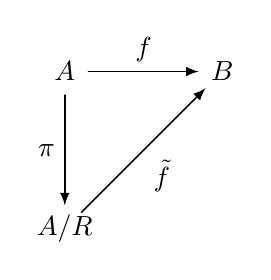
\begin{tikzpicture}[>=latex, line cap=round, line width=0.2mm]
    \coordinate (A) at (0.0,  0.0);
    \coordinate (B) at (2.0,  0.0);
    \coordinate (C) at (0.0, -2.0);

    \node at (A) {$A$};
    \node at (B) {$B$};
    \node at (C) {$A/R$};

    \begin{scope}[->, shorten <=3mm, shorten >=3mm]
        \draw (A) to node [above]       {$f$}         (B);
        \draw (A) to node [left]        {$\pi$}       (C);
        \draw (C) to node [below right] {$\tilde{f}$} (B);
    \end{scope}
\end{tikzpicture}